%--------------------------------
% Fundamentação Teórica 
%-------------------------------
\chapter{Fundamentação Teórica} \label{Fundamentação Teórica}

Este capítulo apresenta os conceitos teóricos que fundamentam o desenvolvimento deste trabalho. Inicialmente são apresentados os princípios relacionados ao fator de potência. Em seguida, são discutidos conceitos de Internet das Coisas (IoT), medição e monitoramento de grandezas elétricas. Por fim, são introduzidos os fundamentos de aprendizado de máquina e redes neurais artificiais, com ênfase na arquitetura Multilayer Perceptron (MLP), utilizada neste trabalho.

\section{Fator de Potência}
O fator de potência (FP) é um importante indicador da eficiência do uso da energia elétrica em sistemas de corrente alternada, expressando a relação entre a potência ativa, efetivamente convertida em trabalho útil, e a potência aparente fornecida pela rede elétrica \cite{Stevenson1994, Glover2012}. Dessa forma, o FP permite avaliar o grau de aproveitamento da energia elétrica consumida por uma instalação, sendo amplamente utilizado como parâmetro técnico para análise da qualidade da energia e do desempenho energético dos sistemas elétricos.

Valores reduzidos de fator de potência indicam a presença significativa de potência reativa no sistema, o que pode resultar em diversos impactos negativos, tais como aumento das perdas elétricas, aquecimento excessivo de condutores, sobrecarga de transformadores, quedas de tensão, subutilização da capacidade instalada e redução da vida útil dos equipamentos \cite{Pansini2011, Mamede2018}. Além disso, no contexto regulatório brasileiro, unidades consumidoras que operam com fator de potência inferior a 0,92 estão sujeitas à cobrança de excedentes de energia reativa, conforme estabelecido pela Agência Nacional de Energia Elétrica (ANEEL), o que eleva os custos operacionais do consumidor.

Em sistemas elétricos de potência, a energia é caracterizada por três tipos fundamentais de potência: ativa, reativa e aparente. A potência ativa, medida em watts (W), corresponde à parcela da potência responsável pela realização de trabalho útil, como movimento mecânico, aquecimento ou iluminação. 

A potência reativa, medida em volt-ampère reativo (VAr), está diretamente associada à defasagem angular entre as formas de onda de tensão e corrente em sistemas de corrente alternada. Essa defasagem ocorre principalmente devido à presença de cargas indutivas, resultando em um consumo adicional de corrente \cite{Glover2012}. Embora não esteja diretamente associada à realização de trabalho útil, é necessária para a criação e manutenção de campos eletromagnéticos em equipamentos como motores e transformadores \cite{Stevenson1994}.

Conforme observado na Fig. \ref{fig:triangulo_potencias}, a combinação vetorial das potências ativa e reativa resulta na potência aparente, medida em volt-ampère (VA), que representa a potência total fornecida pelo sistema elétrico.

\begin{figure}[!htbp]
	\centering
	\caption{Relação entre as potências para o cálculo do fator de potência.}
	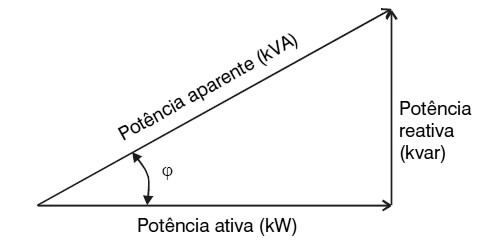
\includegraphics[width=0.6\textwidth]{Figuras/fator-de-potencia-triangulo-das-potencias.jpg}
	\fonte{Adaptado de \citeonline{engeletrica_fp}.}
	\label{fig:triangulo_potencias}
\end{figure}

Matematicamente, o fator de potência pode ser definido como a razão entre a potência ativa ($P$) e a potência aparente ($S$), conforme a Equação \ref{eq:fp}. Este indicador varia em um intervalo de 0 a 1, e quanto maior for a parcela de potência ativa em relação à potência aparente, mais elevado será o fator de potência, indicando maior eficiência energética do sistema.

\begin{equation}
    FP = \cos(\varphi) = \frac{P}{S} \quad \text{ou} \quad \frac{P}{\sqrt{P^{2} + Q^{2}}}
    \label{eq:fp}
\end{equation}

onde $P$ representa a potência ativa, $Q$ a potência reativa, $S$ a potência aparente e $\varphi$ o ângulo de defasagem entre tensão e corrente.


Assim, sistemas operando com fator de potência elevado apresentam menor circulação de corrente para uma mesma demanda de potência ativa, reduzindo perdas elétricas e melhorando o desempenho global da instalação. Por esse motivo, o monitoramento e a correção do fator de potência são práticas fundamentais para a eficiência energética, segurança operacional e conformidade regulatória em unidades consumidoras.

%------------------------------------------------------------------
%------------------------------------------------------------------
\section{Medição e Monitoramento}
A medição e o monitoramento de grandezas elétricas constituem etapas fundamentais para a análise da eficiência energética e da qualidade da energia elétrica em unidades consumidoras. Tradicionalmente, o acompanhamento elétrico em instalações de baixa e média tensão é realizado por meio de instrumentos de medição convencionais ou analisadores de energia, capazes de fornecer informações pontuais ou valores médios sobre o consumo. Entretanto, com a evolução dos sistemas elétricos e o advento do conceito de Redes Elétricas Inteligentes (\textit{Smart Grids}), destacam-se os Medidores Inteligentes (\textit{Smart Meters}), que possibilitam o registro, o armazenamento e a transmissão automatizada de dados elétricos em tempo quase real \cite{MedidoresInteligentes}.

Com o avanço das tecnologias de comunicação e o surgimento do conceito de Internet das Coisas (IoT, do inglês \textit{Internet of Things}), o monitoramento do consumo elétrico passou a ocorrer de forma mais acessível e integrada. Plataformas baseadas em IoT permitem que consumidores acompanhem seus parâmetros de consumo por meio de interfaces online, recebendo notificações e alertas quando determinados limites são atingidos, o que auxilia no controle dos gastos energéticos e na tomada de decisões \cite{GerenciadorMedidorInteligente}. 

Do ponto de vista técnico, a aquisição contínua desses parâmetros mostra-se importante para compreender o comportamento dinâmico das cargas, identificar ineficiências operacionais e detectar anomalias no sistema elétrico, como picos de consumo anormais, que podem indicar falhas ou desperdício de energia \cite{Wang2018}. Entretanto, equipamentos de medição mais avançados geralmente apresentam elevado custo de aquisição e manutenção. 

Nesse contexto, o uso de sensores elétricos de baixo custo associados a plataformas de comunicação IoT tem se tornado uma alternativa viável para a implementação de sistemas de monitoramento em tempo real, possibilitando a coleta contínua de dados que podem ser posteriormente utilizados em modelos de análise e previsão.

%------------------------------------------------------------------
%------------------------------------------------------------------
\section{Internet das Coisas}

O termo Internet das Coisas (\textit{Internet of Things} – IoT) refere-se ao paradigma tecnológico no qual objetos físicos são equipados com sensores, atuadores, capacidade de processamento e comunicação em rede, permitindo que esses dispositivos coletem, transmitam e compartilhem dados por meio da Internet. Nesse contexto, dispositivos conectados passam a interagir entre si e com sistemas computacionais, possibilitando a criação de aplicações capazes de monitorar e controlar processos de forma remota e em tempo real \cite{IoT2015}.

A arquitetura de sistemas IoT geralmente envolve dispositivos de borda (como microcontroladores), protocolos de comunicação (como MQTT, HTTP e CoAP) e plataformas em nuvem ou locais para processamento e visualização dos dados \cite{Majhi2024}. Dispositivos como o ESP8266, de baixo custo e amplamente utilizado para conectividade, permitem a integração de sensores e a transmissão de dados via Wi-Fi, viabilizando aplicações de monitoramento distribuído.

A utilização de IoT tem possibilitado o desenvolvimento de sistemas inteligentes em diferentes áreas, como automação residencial, cidades inteligentes, monitoramento industrial e sistemas de energia. Em aplicações de monitoramento elétrico, dispositivos IoT podem ser utilizados para adquirir grandezas elétricas por meio de sensores e transmiti-las para plataformas de processamento e visualização de dados (como Node-RED, ThingsBoard, etc) \cite{Msane2024, ScientificReports2025}. %Dessa forma, a integração entre sensoriamento, comunicação em rede e processamento de dados permite o desenvolvimento de soluções capazes de monitorar e analisar o comportamento de sistemas elétricos em tempo real \cite{Msane2024, ScientificReports2025}.

%------------------------------------------------------------------
%------------------------------------------------------------------
\section{Aprendizado de Máquina}
O Aprendizado de Máquina (ML, do inglês \textit{Machine Learning}) é uma área da Inteligência Artificial (IA) dedicada ao desenvolvimento de métodos computacionais capazes de aprender a partir de dados, sem a necessidade de serem explicitamente programados para cada tarefa específica \cite{Samuel1959}. Esses métodos utilizam algoritmos que identificam padrões e regularidades em conjuntos de dados e os representam por meio de modelos matemáticos, os quais podem ser posteriormente utilizados para realizar inferências ou previsões sobre novos dados \cite{1deepLearningTempestade}.

De modo geral, o Aprendizado de Máquina pode ser classificado em quatro categorias principais, conforme ilustrado na Figura \ref{fig:tipos de aprendizado de maquina}: aprendizado supervisionado, no qual o modelo é treinado a partir de dados rotulados; aprendizado não supervisionado, que busca identificar estruturas ou padrões em dados não rotulados; aprendizado semi-supervisionado, que combina dados rotulados e não rotulados; e o aprendizado por reforço, baseado na interação de um agente com o ambiente por meio de recompensas e penalidades \cite{nambundo2025}.

Durante o processo de aprendizado, o modelo ajusta iterativamente seus parâmetros internos com o objetivo de minimizar erros ou maximizar métricas de desempenho associadas à tarefa em questão. Dessa forma, o sistema é capaz de aprimorar sua capacidade de generalização, ou seja, de produzir respostas adequadas mesmo diante de dados não previamente observados \cite{Sarker2021}.

\begin{figure}[!htbp]
	\centering
	\caption{Categorias do aprendizado de máquina.}
	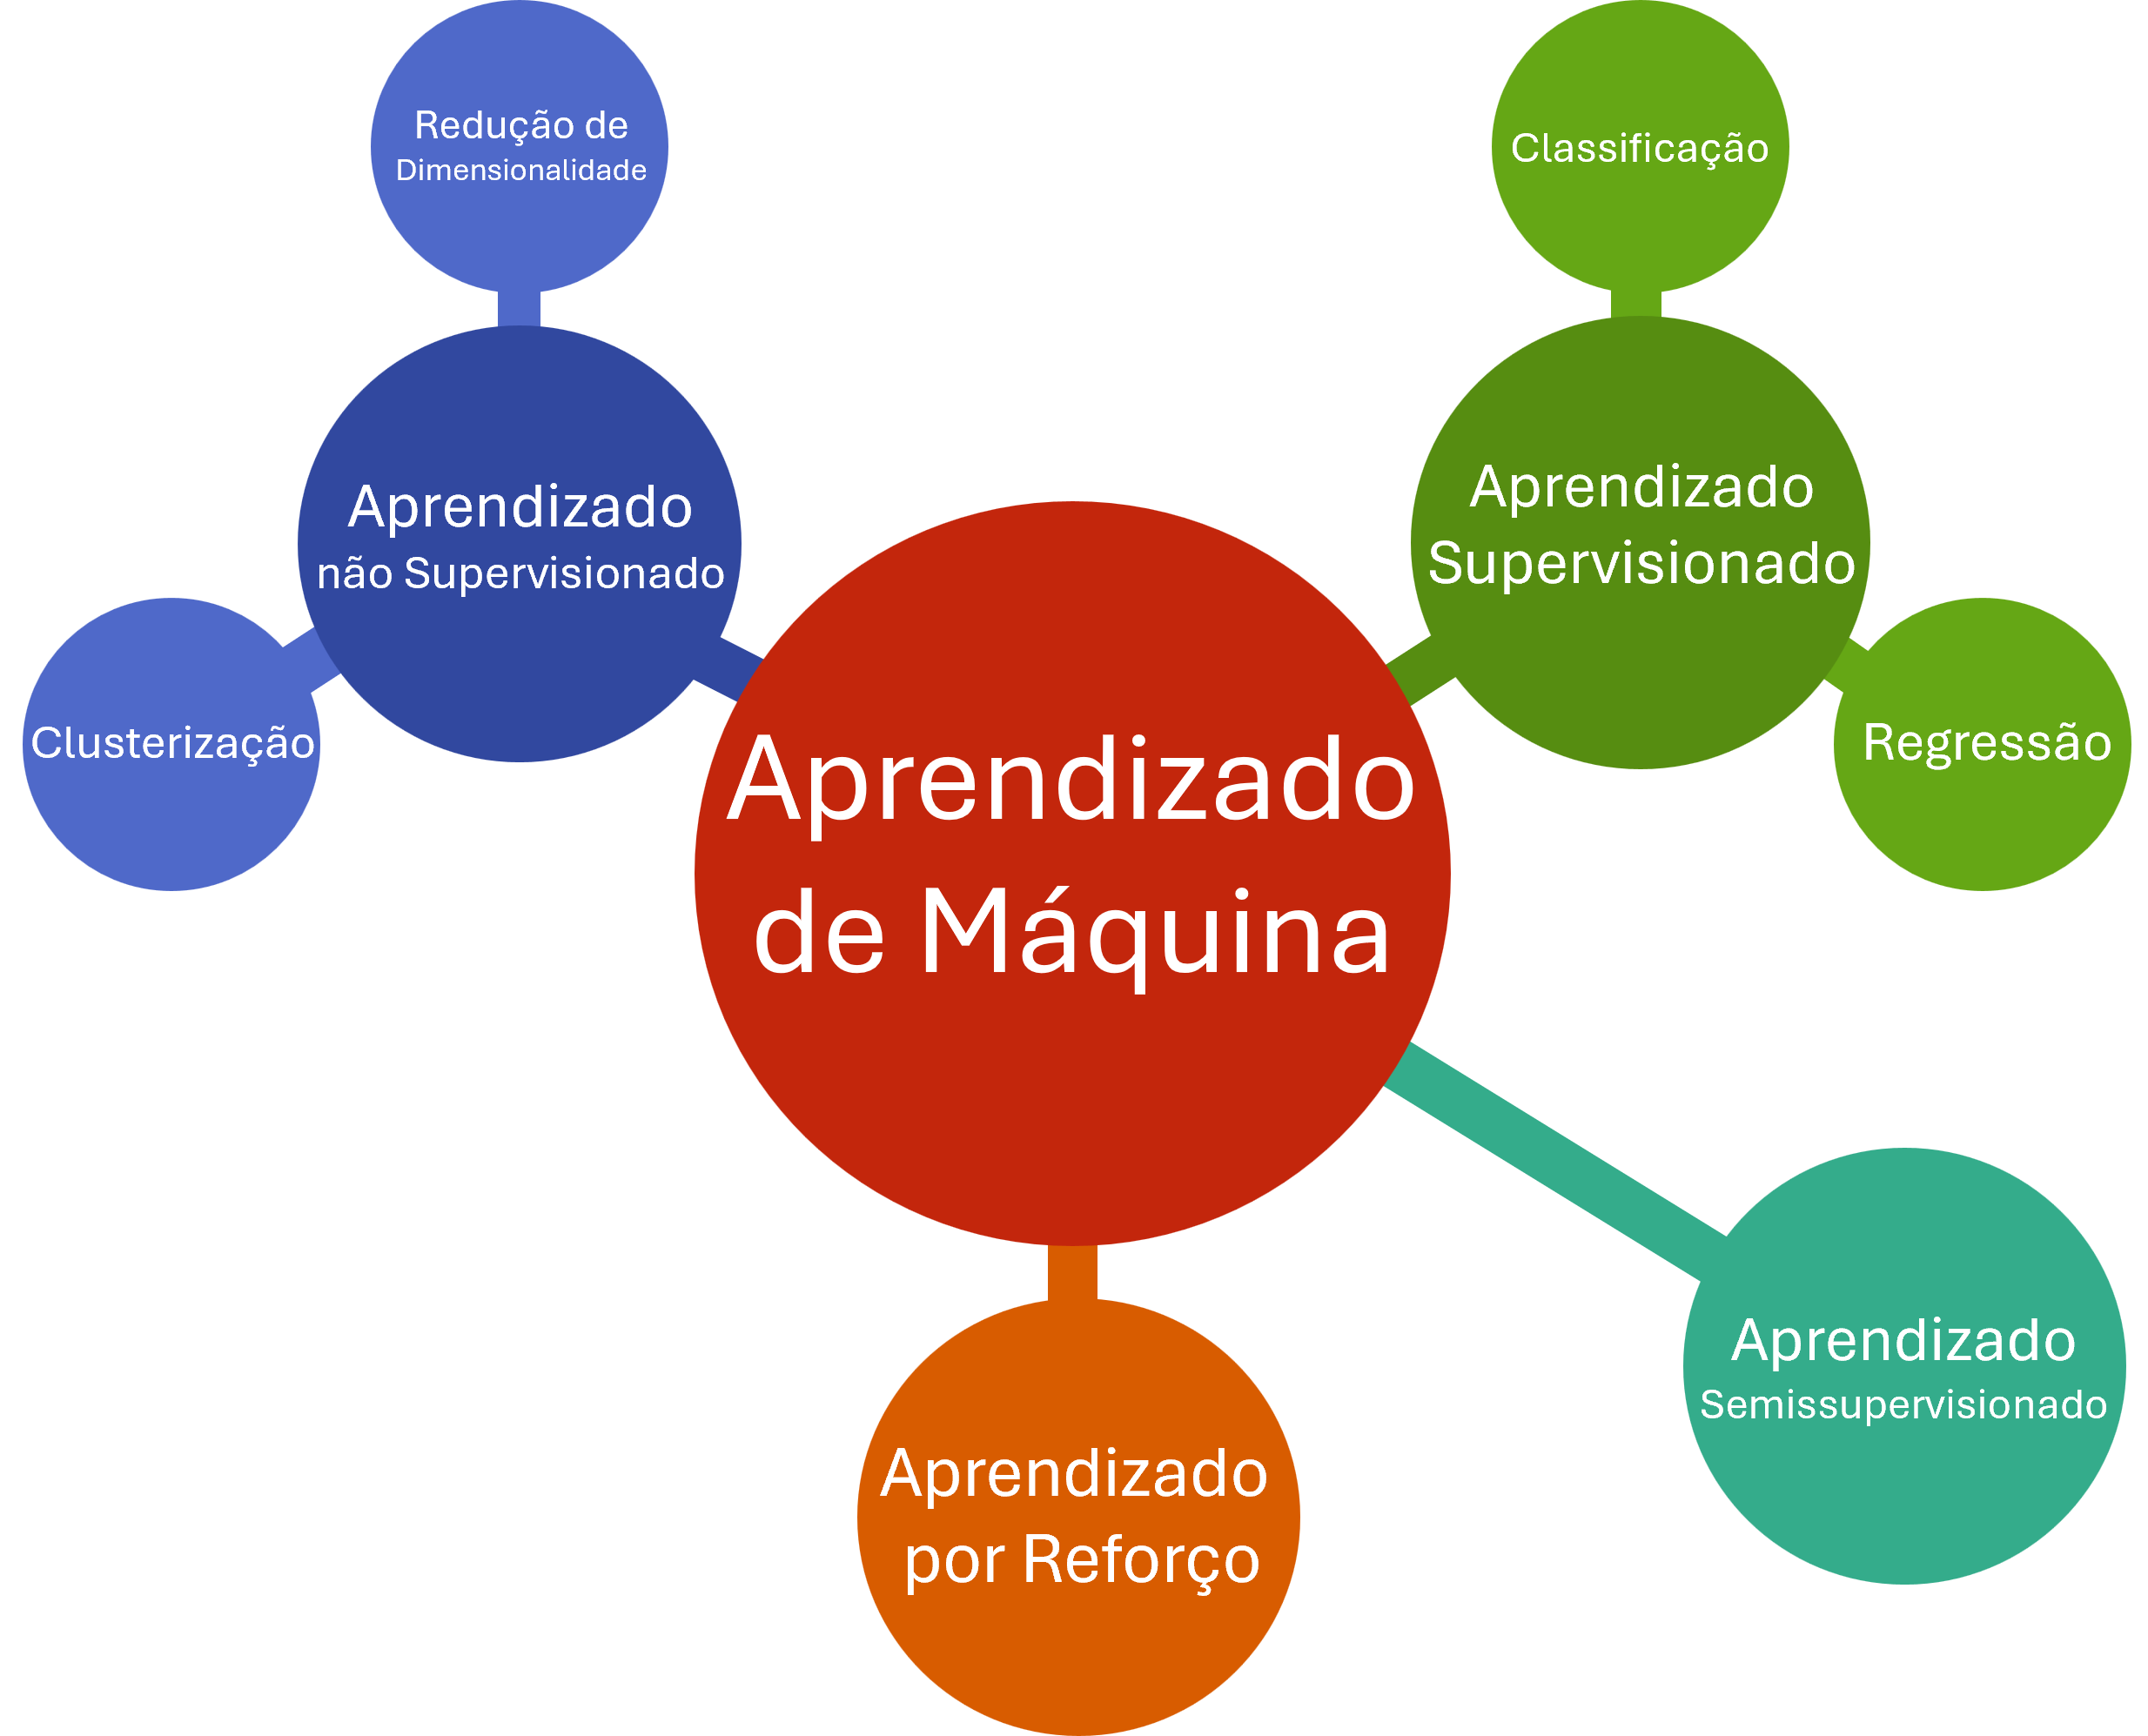
\includegraphics[width=0.83\textwidth]{Figuras/areas_ML (3).png}
	\fonte{Adaptado de \citeonline{TwipeML}.}
	\label{fig:tipos de aprendizado de maquina}
\end{figure}

Entre os diversos algoritmos desenvolvidos no contexto do aprendizado de máquina, as redes neurais artificiais têm se destacado ao longo dos anos devido à sua estrutura flexível e à capacidade de modelar relações não lineares complexas \cite{Bishop1994}. Essas características tornam as redes neurais especialmente adequadas para aplicações em problemas de classificação e regressão, abrangendo desde arquiteturas mais simples até modelos mais profundos e sofisticados \cite{Sarker2021}.

\subsection{Aprendizado de Máquina Supervisionado}
% É o termo geral utilizado para modelos nos quais os dados de treinamento incluem tanto valores de características quanto valores de rótulos conhecidos
% que são treinados a partir de um conjunto de dados rotulados, ou seja, onde os valores de entrada (características) estão associados a um valor de saída conhecido (rótulo) \cite{microsoft_classificacao}.

Conforme ilustrado na Figura \ref{fig:tipos de aprendizado de maquina}, o aprendizado de máquina supervisionado pode ser dividido em duas principais categorias:

\begin{itemize}
    \item \textbf{Classificação}: a variável de saída é qualitativa, assumindo valores discretos que representam categorias ou classes. O objetivo é aprender uma fronteira de decisão que permita atribuir cada nova observação a uma categoria específica. Quando existem apenas duas classes possíveis, o problema é denominado classificação binária, para três ou mais categorias, trata-se de classificação multiclasses \cite{codecademy_classification, microsoft_classificacao}.
    
    \item \textbf{Regressão}: a variável de saída é quantitativa, assumindo valores contínuos. O objetivo é modelar a relação entre as variáveis de entrada e um valor numérico a ser estimado. A regressão busca encontrar uma função que melhor represente a tendência dos dados, minimizando o erro entre os valores previstos e os reais \cite{ibm_regressao}.
\end{itemize}

% \begin{figure}[!htbp]
%     \centering
%     \caption{Principais categorias do aprendizado supervisionado.}
%     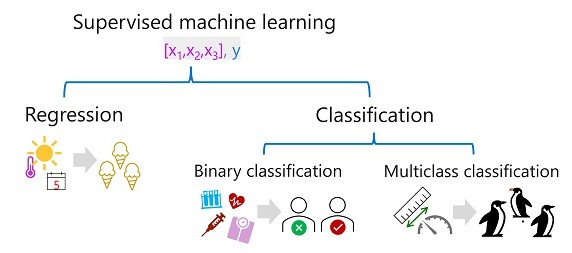
\includegraphics[scale=0.7]{Figuras/supervised-machine-learning-types.jpg}
%     \fonte{Adaptado de \citeonline{microsoft_classificacao}.}
%     \label{fig:tipos_aprendizado_supervisionado}
% \end{figure}

A Tabela \ref{tab:comparacao_class_reg} sintetiza as principais diferenças entre as duas abordagens.

\begin{table}[h]
    \centering
    \caption{Comparação entre classificação e regressão}
    \label{tab:comparacao_class_reg}
    \begin{tabular}{lcc}
    \hline
    \textbf{Característica} & \textbf{Classificação} & \textbf{Regressão} \\
    \hline
    Tipo da saída & Discreta (categórica) & Contínua (numérica) \\
    Objetivo & Atribuir a uma classe & Estimar um valor \\
    Exemplos & Tipo de carga, diagnóstico médico & Preço, temperatura, FP \\
    Métricas de avaliação & Acurácia, precisão, recall, F1-score & MSE, MAE, RMSE, R² \\
    \hline
    \end{tabular}
    \fonte{Adaptado de \citeonline{geeks_class_reg}.}
\end{table}



%------------------------------------------------------------------
%------------------------------------------------------------------
\section{Redes Neurais Artificiais}

As Redes Neurais Artificiais (RNAs) são modelos computacionais amplamente utilizados no contexto do Aprendizado de Máquina, inspirados no funcionamento do sistema nervoso biológico que adquirem conhecimento através da experiência \cite{NEGNEVITSKY2005}. Esses modelos são constituídos por um conjunto de unidades de processamento interconectadas, denominadas neurônios artificiais, cujas conexões, chamadas de sinapses, são associadas a pesos ajustáveis para transmissão das informações entre os demais neurônios. Por meio do ajuste desses pesos durante o processo de aprendizagem, as RNAs são capazes de adquirir conhecimento a partir de dados, armazenando-o de forma distribuída na rede \cite{IvanSilva2010}.

De modo geral, as RNAs apresentam características importantes, como capacidade de adaptação, generalização, aprendizado a partir de exemplos e tolerância a ruídos, o que as torna especialmente adequadas para problemas complexos envolvendo relações não lineares, como classificação, regressão e previsão de séries temporais. Em razão dessas propriedades, as redes neurais constituem uma das principais técnicas dentro do campo do Aprendizado de Máquina, o qual, por sua vez, integra o domínio mais amplo da Inteligência Artificial, conforme ilustrado na Figura \ref{fig:hierarquiaIA}.

\begin{figure}[!htbp]
	\centering
	\caption{Organização das principais áreas da Inteligência Artificial.}
	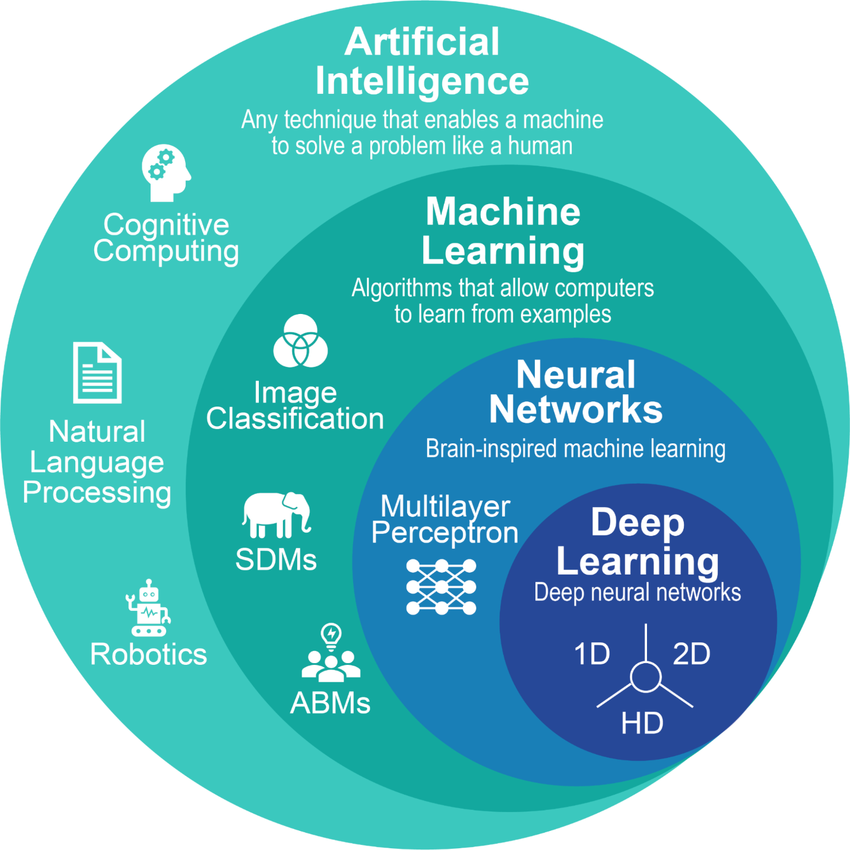
\includegraphics[width=0.47\textwidth]{Figuras/hierarquiaIA.png}
	\fonte{Adaptado de \cite{AI_Landscape_Ecology_2024}.}
	\label{fig:hierarquiaIA}
\end{figure}

% Os primeiros estudos formais sobre redes neurais artificiais remontam à década de 40, com os trabalhos de Warren S. McCulloch e Walter Pitts, que propuseram um modelo matemático simplificado do neurônio biológico e demonstraram como seu comportamento poderia ser representado artificialmente \cite{MCCULLOCH1943}. Posteriormente, em 1949, Donald Hebb introduziu o conceito de aprendizado em redes neurais por meio do ajuste das conexões sinápticas, em seu trabalho intitulado \textit{“The organization of Behavior”}, defendendo que o fortalecimento dessas conexões ocorre quando neurônios são ativados simultaneamente, princípio que ficou conhecido como regra de Hebb \cite{Passos2017}.

% Em 1958, Frank Rosenblatt apresentou o \textit{perceptron}, considerado o primeiro modelo de rede neural artificial capaz de ser treinado para a classificação de padrões por meio do ajuste iterativo dos pesos sinápticos \cite{ROSENBLATT1958}. O \textit{perceptron} pertence à classe das arquiteturas do tipo \textit{feedforward} e caracteriza-se por sua simplicidade estrutural, uma vez que é constituído por apenas uma camada com um único neurônio \cite{Vinicius2017}. Esse modelo representou um marco no desenvolvimento das RNAs ao demonstrar a viabilidade do aprendizado supervisionado em sistemas artificiais, embora apresente limitações na resolução de problemas que não são linearmente separáveis. 

Os primeiros estudos sobre redes neurais artificiais surgiram na década de 1940. Warren S. McCulloch e Walter Pitts (1943) propuseram um modelo matemático do neurônio biológico, enquanto Hebb (1949) introduziu o princípio de aprendizado por meio de ajustes das conexões sinápticas, conhecido como regra de Hebb \cite{MCCULLOCH1943, Passos2017}, defendendo que o fortalecimento dessas conexões ocorre quando neurônios são ativados simultaneamente. Em 1958, Frank Rosenblatt apresentou o \textit{perceptron}, primeiro modelo de rede neural capaz de aprendizado supervisionado por ajuste iterativo dos pesos \cite{ROSENBLATT1958}. Embora limitado a problemas linearmente separáveis, o \textit{perceptron} consolidou a viabilidades do aprendizado de máquina supervisionado \cite{Vinicius2017}.

As redes neurais artificiais podem ser classificadas de acordo com sua arquitetura e com a forma de conexão entre os neurônios. Dentre as principais categorias, destacam-se as redes do tipo \textit{feedforward}, nas quais o fluxo de informação ocorre em uma única direção, da camada de entrada até a camada de saída; as redes recorrentes, caracterizadas pela realimentação das saídas como entradas para outros neurônios, permitindo a modelagem de dependências temporais; e as redes com conexões simétricas, que considera a disposição espacial dos neurônios para o ajuste dos pesos e limiares \cite{ArquiteturasRNA}.

Independentemente da arquitetura, um neurônio artificial é composto por elementos básicos comuns, conforme ilustrado na Figura \ref{fig:representacao_neuronio_artificial}. De acordo com \cite{HAYKIN2001}, esses elementos incluem: sinais de entrada $(x_i)$, pesos sinápticos $(w_i)$, um somador para a combinação linear das entradas, um termo de bias $(b)$ e uma função de ativação $g(\cdot)$, responsável por introduzir não linearidade ao modelo. A saída resultante desse processo é o sinal $(y)$ do neurônio.


% Segundo \cite{HAYKIN2001}, os principais componentes de um neurônio artificial são:
% \begin{itemize}
%     \item Sinais de entrada $(x_i)$: representam os sinais externos que alimentam o modelo, geralmente provenientes de dados normalizados ou previamente processados;
    
%     \item Pesos sinápticos $(w_i)$: são valores ajustados durante o treinamento da rede neural, responsáveis por ponderar a influência de cada sinal de entrada no neurônio;
    
%     \item Somador $(\sum)$: responsável pelo cálculo da soma ponderada das entradas, realizando a combinação linear entre os sinais de entrada e seus respectivos pesos;
    
%     \item Bias ou viés $(b)$: parâmetro adicional que permite deslocar a função de ativação, atuando como um termo independente na soma ponderada, possibilitando maior flexibilidade ao modelo e permitindo que o neurônio seja ativado mesmo quando todas as entradas possuem valor nulo;

%     \item Potencial de ativação $(u)$: resultado da combinação linear das entradas ponderadas acrescida do termo de bias, sendo este valor o argumento da função de ativação. Quando $u \geq 0$, o neurônio tende a produzir um potencial excitatório; caso contrário, o potencial é considerado inibitório;

%     \item Função de ativação $(g(\cdot))$: aplicada ao potencial de ativação, tem como objetivo introduzir não linearidade no modelo e limitar o valor do sinal de saída, geralmente em intervalos como $(0,1)$ ou $(-1,1)$;
    
%     \item Sinal de saída $(y)$: corresponde ao valor final produzido pelo neurônio, podendo ser utilizado como entrada para outros neurônios em camadas subsequentes da rede.
% \end{itemize}

% O modelo matemático de um neurônio artificial, com seus componentes fundamentais, é ilustrado na Figura \ref{fig:representacao_neuronio_artificial}. Nessa representação, observa-se um conjunto de entradas $(x_i)$ que, ao serem multiplicadas por seus respectivos pesos $(w_i)$ e posteriormente somadas, geram um sinal interno que é então aplicado a uma função de ativação que, por sua vez, é responsável por determinar o nível de ativação do neurônio, produzindo o sinal de saída da unidade neural.

\begin{figure}[!htbp]
	\centering
	\caption{Modelo de um neurônio artificial.}
	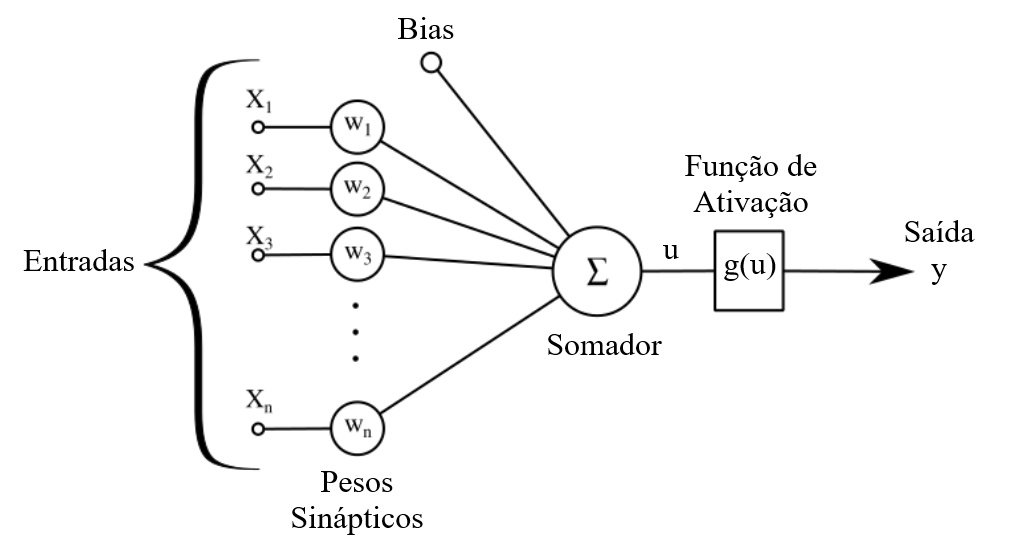
\includegraphics[width=0.8\textwidth]{Figuras/Modelo_Neuronio_Artificial.png}
	\fonte{Adaptado de \citeonline{Azevedo2016}.}
	\label{fig:representacao_neuronio_artificial}
\end{figure}

Assim, a operação matemática realizada por um neurônio artificial pode ser descrita pela Equação \ref{eq:neuronio}.

\begin{equation}
    y = g\left(\sum_{i=1}^{n} w_i x_i + b \right)
    \label{eq:neuronio}
\end{equation}

%------------------------------------------------------------------
%------------------------------------------------------------------
\subsection{Rede Neural \textit{Multilayer Perceptron (MLP)}}

A arquitetura \textit{Multilayer Perceptron (MLP)} surgiu como extensão do \textit{Perceptron} de Rosenblatt para superar sua limitação na resolução de problemas não linearmente separáveis \cite{ROSENBLATT1958, Minsky1969}. Sua principal inovação é a inclusão de uma ou mais camadas ocultas entre as camadas de entrada e saída, permitindo a representação de funções não lineares complexas, conforme ilustrado na Figura \ref{fig:representacao_mlp}.

A MLP é uma rede neural do tipo \textit{feedforward}, na qual a informação flui unidirecionalmente da entrada para a saída, sem realimentação \cite{HAYKIN2001}. Sua arquitetura básica, ilustrada na Figura \ref{fig:representacao_mlp}, é composta por três tipos de camadas:
\begin{itemize}
    \item \textbf{Camada de entrada}: responsável por receber os dados;
    \item \textbf{Camadas ocultas}: realizam transformações não lineares por meio de funções de ativação;
    \item \textbf{Camada de saída}: fornece a resposta final do modelo.
\end{itemize}

O aprendizado da MLP ocorre de forma supervisionada, ajustando os pesos sinápticos e \textit{biases} para minimizar uma função de custo, que mede o erro entre a saída estimada e o valor desejado \cite{Arquiteturadasredes}. O algoritmo mais empregado para esse fim é a retropropagação do erro (\textit{backpropagation}), que calcula os gradientes da função de custo em relação aos pesos e os ajusta por meio do gradiente descendente ou de suas variações. O erro é propagado da camada de saída para as camadas anteriores, permitindo o ajuste iterativo dos pesos sinápticos \cite{Rumelhart1986}. Outras abordagens, como métodos evolucionários, também podem ser utilizadas, dependendo das características do problema \cite{Bishop1994, HAYKIN2001}.

A MLP é amplamente utilizada em problemas de regressão e previsão de séries temporais devido à sua capacidade de aproximar funções contínuas não lineares. Essa propriedade é garantida pelo Teorema da Aproximação Universal, que estabelece que redes \textit{feedforward} com ao menos uma camada oculta e funções de ativação adequadas podem aproximar qualquer função contínua em compactos com erro arbitrariamente pequeno \cite{Cybenko1989, Hornik1989}. Ao utilizar valores passados como entrada, a MLP captura dependências temporais implícitas, sendo eficaz na modelagem de grandezas dinâmicas como demanda de energia e fator de potência \cite{Amjady2009, Andrade2015}.

Essa capacidade de modelagem não linear torna a MLP particularmente adequada para sistemas elétricos, onde variáveis como potência, corrente e fator de potência apresentam comportamento dinâmico e não linear. Além disso, sua estrutura relativamente simples, comparada a arquiteturas mais complexas, resulta em menor custo computacional durante a inferência, favorecendo sua aplicação em sistemas com recursos limitados \cite{Sarker2021}.

\begin{figure}
\caption{Rede Neural \textit{feedforward Multilayer Perceptron}.}
 \centering   
\begin{tikzpicture}[
  >={Stealth[length=3mm]},
  line/.style={->, thick},
  conn/.style={->, gray!40, thin},
  inNode/.style={
    draw=orange!80!brown, fill=orange!20,
    minimum size=6mm, rounded corners=2pt
  },
  hidNode/.style={
    circle, draw=blue!60!black, fill=blue!12,
    minimum size=11mm
  },
  outNode/.style={
    circle, draw=teal!70!black, fill=teal!18,
    minimum size=11mm
  }
]

% --- Nós de entrada ---
\node[inNode] (I1) at (0, 2.4) {};
\node[inNode] (I2) at (0, 1.2) {};
\node[inNode] (I3) at (0, -0.4) {};
\node at (0, 0.62) {\large $\vdots$};

% --- Camada oculta 1 ---
\node[hidNode] (H11) at (3, 2.4) {};
\node[hidNode] (H12) at (3, 1.2) {};
\node[hidNode] (H13) at (3, -0.4) {};
\node at (3, 0.5) {\large $\vdots$};

% --- Camada oculta 2 ---
\node[hidNode] (H21) at (6, 2.4) {};
\node[hidNode] (H22) at (6, 1.2) {};
\node[hidNode] (H23) at (6, -0.4) {};
\node at (6, 0.5) {\large $\vdots$};

% --- Nós de saída ---
\node[outNode] (O1) at (9, 1.8) {};
\node[outNode] (O2) at (9, 0.6) {};

% --- Conexões entrada -> oculta 1 ---
\foreach \i in {1,2,3}{
  \foreach \j in {1,2,3}{
    \draw[conn] (I\i) -- (H1\j);
  }
}

% --- Conexões oculta 1 -> oculta 2 ---
\foreach \i in {1,2,3}{
  \foreach \j in {1,2,3}{
    \draw[conn] (H1\i) -- (H2\j);
  }
}

% --- Conexões oculta 2 -> saída ---
\foreach \i in {1,2,3}{
  \foreach \j in {1,2}{
    \draw[conn] (H2\i) -- (O\j);
  }
}

% --- Setas de entrada ---
\draw[line, orange!80!brown] (-1.3, 2.4) -- (I1)
  node[midway, above, font=\small] {$x_1$};
\draw[line, orange!80!brown] (-1.3, 1.2) -- (I2)
  node[midway, above, font=\small] {$x_2$};
\draw[line, orange!80!brown] (-1.3, -0.4) -- (I3)
  node[midway, above, font=\small] {$x_n$};

% --- Setas de saída ---
\draw[line, teal!70!black] (O1) -- ++(1.3, 0)
  node[right, font=\small] {$\hat{y}_1$};
\draw[line, teal!70!black] (O2) -- ++(1.3, 0)
  node[right, font=\small] {$\hat{y}_2$};

% --- Chave sobre camadas ocultas ---
\draw[decorate, decoration={brace, amplitude=5pt}, blue!60!black]
  (2.2, 3.1) -- (6.8, 3.1)
  node[midway, above=5pt, font=\small\bfseries, blue!70!black]
  {Camadas ocultas};


% --- Legenda em linha ---
\node[inNode,  minimum size=3.5mm] at (1.2, -1.4) {};
\node[anchor=west, font=\scriptsize] at (1.45, -1.41) {Camada de entrada};

\node[hidNode, minimum size=4mm]   at (4.5, -1.4) {};
\node[anchor=west, font=\scriptsize] at (4.75, -1.4) {Camadas ocultas};

\node[outNode, minimum size=4mm]   at (7.5, -1.4) {};
\node[anchor=west, font=\scriptsize] at (7.75, -1.4) {Camada de saída};

\draw[gray!50, thin, rounded corners=2pt]
  (0.7, -1.8) rectangle (10.5, -1.1);


\end{tikzpicture}
\label{fig:representacao_mlp}
 \fonte{\me{2026}} 

\end{figure}

